\subsection{Trainings- und Testdaten}
\begin{lstlisting}[label=lst:sampleGesture,caption={Beispiel einer gespeicherten Handgeste von Links nach Rechts.}]
    ...
    665,683,669,690,627,670,672,611,557,1
    662,679,657,676,564,592,633,467,415,1
    645,653,583,627,549,483,598,474,230,1
    576,444,269,488,251,209,352,184,187,1
    361,254,123,343,130,82,304,83,36,1
    131,69,41,120,34,39,72,25,30,1
    49,71,174,61,45,206,40,45,110,1
    111,242,473,113,195,467,122,210,343,1
    272,559,637,304,518,639,401,553,562,1
    566,646,654,592,580,654,634,618,602,1
    ...
\end{lstlisting}
\begin{figure}
    \centering
    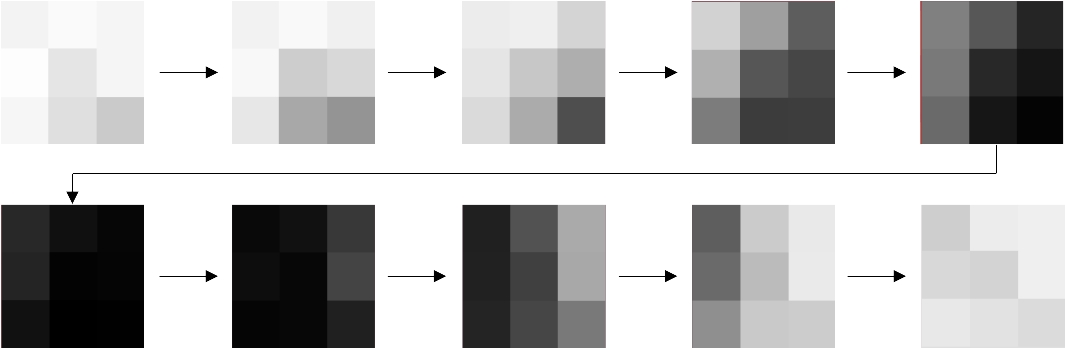
\includegraphics[width=\linewidth]{images/sample_gesture_total.jpg}
    \caption{Illustration der Handgeste von Links nach Rechts aus Listing \ref{lst:sampleGesture}.}
    \label{fig:sample_gesture}
\end{figure}
Die Modelle werden auf Basis von aufgenommenen Daten trainiert und getestet. Jedes aufgenommene Bild wird durch einen Komma separierten Vektor von Zahlen dargestellt gefolgt von einer Annotation für den Gestentyp.
Eine Geste ist eine Folge von Bildern, die die gleiche Annotation teilen (siehe Listing \ref{lst:sampleGesture}). Insgesamt gibt es 4792 Aufnahmen von validen Handgesten, die unter verschiedenen Lichtverhältnissen
und Distanzen zur Kamera aufgenommen wurden. Dabei wurde die Gesten mit der Hand und Finger ausgeführt in verschiedenen Geschwindigkeiten (TODO: Quelle?!).
\subsubsection{Synthetische Daten}
Um die Datenmenge zu erhöhen, können synthetisch Daten aus den bestehenden Daten erzeugt werden indem sie rotiert werden, Rauschen hinzugefügt wird oder die Helligkeit, Kontraste oder
Gamma verändert wird \cite{venzkeArticle}.
\subsubsection{Testdaten und Metrik von Klisch}
Als Testdaten wird ein Teil der Datenmenge bezeichnet, die nicht zum trainieren verwendet wurde. Kubik hat Testdaten unter verschiedenen Lichtverhältnissen und Entfernungen zur Kamera aufgenommen. Klisch hat
daraus eine Testmenge erstellt die von Klisch und Giese zur Verifikation verwendet wurden \cite{klischThesis, gieseThesis}. Klisch definiert die Erkennungsgenauigkeit als Verhältnis zwischen der Anzahl an korrekt
erkannten Gesten und der Gesamtanzahl (siehe Formel \ref{klisch_metric}) \cite{klischThesis}.
\begin{align}
    accuracy = \frac{\#true\ positives}{\#total\ gestures}
    \label{klisch_metric}
\end{align}
